\documentclass[a4paper,11pt]{jsarticle}


% 数式
\usepackage{amsmath,amsfonts}
\usepackage{bm}
\usepackage{physics}
% 画像
\usepackage[dvipdfmx]{graphicx}
% ローマ数字
\usepackage{otf}
% 単位
\usepackage{siunitx}
% 表
\usepackage{multirow}
% 化学反応
\usepackage[version=4]{mhchem}
% 引用
\usepackage{url}

\begin{document}

\title{アロステリック制御}
\author{生物物理班 齋藤駿一}
\date{\today}
\maketitle

\tableofcontents

\section{はじめに}
生物の細胞には様々な機能が備わっている.
まず,細胞は分裂して自分のコピーを作り出すことができる.
また,多細胞生物の場合,細胞は周囲の状況から自分の役割を認識し,それに特化した細胞に分化することがある.
ほかにも,大腸菌やゾウリムシなどの場合,べん毛や繊毛を振り回して水中を泳ぐことができる.

こうした機能は決して天から降ってきたものではなく,細胞内の化学反応によって綿密に制御されている.
一般に細胞は,何らかの物質(リガンド)の濃度を感知し,それに応じて適切に振る舞いを制御している.
ここで,リガンドの濃度を感知するため,細胞はリガンドと結合する部分(サイト)を持つ受容体を用いる.
つまり,リガンドが多いほど受容体のサイトはリガンドで埋まっていくはずなので,逆に受容体のサイトがどれだけ埋まっているか(占有率)をもとにリガンドの濃度を知ることができる.
受容体のサイトの占有率は,受容体とリガンドの複合体から発される信号や,受容体が酵素として働く反応への影響などを通して,細胞の振る舞いを変化させる.

では,リガンドの濃度と受容体のサイトの占有率の関係は具体的にどうなっているのだろうか.
本稿では,参考文献\cite{TBoC}をもとに,リガンドと受容体の結合の仕方を3通り考える.
そしてその各々について,数式を用いて定量的に議論する.

\section{最も単純な反応}
まず,受容体Yが1つだけ結合サイトを持ち,そこにリガンドXが結合する場合を考える.
このときの化学反応式は
\begin{equation}
  \ce{X + Y <=>[$k$_{on}][$k$_{off}] XY}
\end{equation}
となる.
ここで,矢印の上についている文字は正反応(左から右への反応)の速度定数を表し,矢印の下についている文字は逆反応(右から左への反応)の速度定数を表す.
この反応のレート方程式は,
\begin{equation}
  \dv{t}[\ce{XY}] = k_{\mathrm{on}}[\ce{X}][\ce{Y}] - k_{\mathrm{off}}[\ce{XY}]
\end{equation}
となる.
定常状態ではどの物質の濃度も変化しなくなるので,上式の左辺は0となる.
したがって
\begin{equation}
  \frac{[\ce{X}][\ce{Y}]}{[\ce{XY}]} = \frac{k_{\mathrm{off}}}{k_{\mathrm{on}}}
\end{equation}
を得る.
この量は解離定数と呼ばれる定数である:
\begin{equation}
  K_d = \frac{k_{\mathrm{off}}}{k_{\mathrm{on}}}
\end{equation}
ここで受容体分子の総濃度を
\begin{equation}
  [\ce{Y_{total}}] = [\ce{Y}] + [\ce{XY}]
\end{equation}
とし,これを一定と見なす.
すると,受容体の結合サイトの占有率$p$は
\begin{equation}
  p = \frac{[\ce{XY}]}{[\ce{Y_{total}}]} = \frac{[\ce{X}]}{K_d + [\ce{X}]} \label{normal}
\end{equation}
と分かる.

\begin{figure}[htbp]
  \centering
  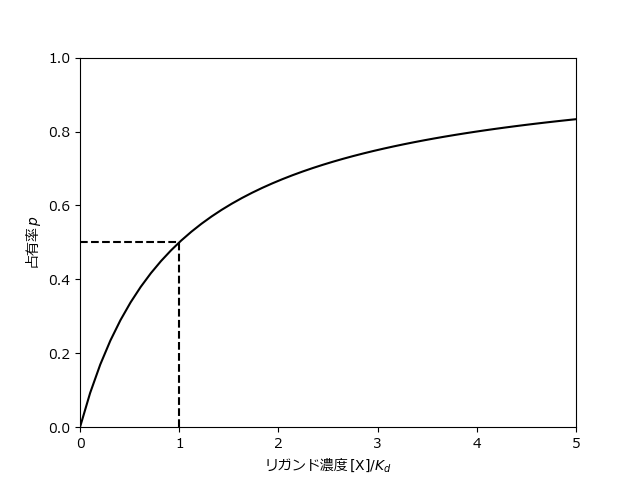
\includegraphics[width=10cm]{simple.png}
  \caption{最も単純なモデルで得られる曲線}
  \label{fig:simple}
\end{figure}

この式\eqref{normal}をプロットしてみると,図\ref{fig:simple}のような双曲線が得られる.
この図から,リガンド濃度が増えると受容体は埋まっていき,占有率が頭打ちになっていく(飽和する)ことが分かる.


\section{Hillの式とアロステリック効果}
しかし,実際には式\eqref{normal}に当てはまらない反応が多く確認されている.
生命活動を制御する際には,リガンドの濃度に対して受容体のサイトの占有率がスイッチ的に(ONかOFFかはっきり)応答することが望ましい場合がある\cite{PBoC}.
式\eqref{normal}のような関数では,ON(受容体のサイトが飽和した状態)とOFF(受容体のサイトがガラ空きの状態)の中間の濃度領域が広すぎるのである.

そこで,受容体Yが$n$個の結合サイトを持ち,そのすべてに1個ずつ,リガンドが一斉に結合するような状況を考える.
化学反応式で書くと,
\begin{equation}
  \ce{$n$X + Y <=>[$k$_{on}][$k$_{off}] X_{$n$}Y}
\end{equation}
のようになる.
このときレート方程式は
\begin{equation}
  \dv{t}[\ce{X_{n}Y}] = k_{\mathrm{on}}[\ce{X}]^n[\ce{Y}] - k_{\mathrm{off}}[\ce{X_{n}Y}]
\end{equation}
で与えられる.
これより,定常状態では
\begin{equation}
  \frac{[\ce{X}]^n[\ce{Y}]}{[\ce{X_{n}Y}]} = \frac{k_{\mathrm{off}}}{k_{\mathrm{on}}} = K_d^n
\end{equation}
となる.
ただしここでは$K_d$の$n$乗を解離定数とした.
よって,受容体分子の総濃度を
\begin{equation}
  [\ce{Y_{total}}] = [\ce{Y}] + [\ce{X_{n}Y}]
\end{equation}
と書いて,これを一定と見なすと,受容体の結合サイトの占有率は
\begin{equation}
  p = \frac{[\ce{X_{n}Y}]}{[\ce{Y_{total}}]} = \frac{[\ce{X}]^n}{K_d^n + [\ce{X}]^n} \label{hill}
\end{equation}
となる.

\begin{figure}[htbp]
  \centering
  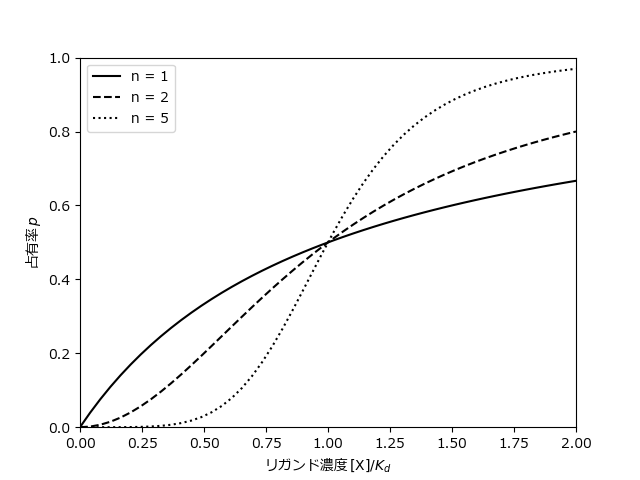
\includegraphics[width=10cm]{hill.png}
  \caption{Hillの式から得られる曲線}
  \label{fig:hill}
\end{figure}

次に式\eqref{hill}を考察する.
$n=1$のときは先ほどの場合とまったく同じだが,$n$を増やすとどうなるだろうか.
計算して確かめると,占有率のグラフはリガンド濃度に対してS字型になることが分かる.
このようなS字型の曲線はシグモイド曲線と呼ばれる.
また,$n$を大きくするほどS字カーブが急峻になることが分かる.
つまり,この$n$を大きくすることで,リガンドの濃度に対するスイッチ的な応答が実現する.

また,Hillの式を導くにあたって,受容体のとりうる状態として$\ce{Y}$と$\ce{X_{$n$}Y}$の二つしか考えなかった.
この状況は,受容体はリガンドが一つ結合した時点で,残りのサイトすべてにリガンドを結合するしかなくなるともいえる.
つまり,リガンドの結合により受容体の状態が変わり,受容体とリガンドが大幅に結合しやすくなったという見方ができる.
このように,受容体のサイトが複数あるとき,あるサイトに何かが結合することで別のサイトでの結合に影響が出ることをアロステリック効果という.


\section{Hillプロット}
また,式\eqref{hill}を変形すると
\begin{equation}
  \qty(\frac{[\ce{X}]}{K_d})^n = \frac{p}{1-p}
\end{equation}
となり,この両辺の対数をとると
\begin{equation}
  \log{\frac{p}{1-p}} = n\qty(\log{[\ce{X}]} - \log{K_d})
\end{equation}
が分かる.
したがって,リガンド濃度$[\ce{X}]$を横軸(x軸)にとり,占有率の高さを表すパラメータ$p/(1-p)$を縦軸(y軸)にとって両対数表示すると,Hillの式に従う場合は直線となる.
また,その直線の傾きは$n$,$p/(1-p)$が1になるときのリガンド濃度は$K_d$となる.
このようなグラフをHillプロットという.
実験結果をもとにこのHillプロットを行うと,測定に使ったリガンドと受容体の振る舞いをHillの式と比較して議論できる.

\begin{figure}[htbp]
  \centering
  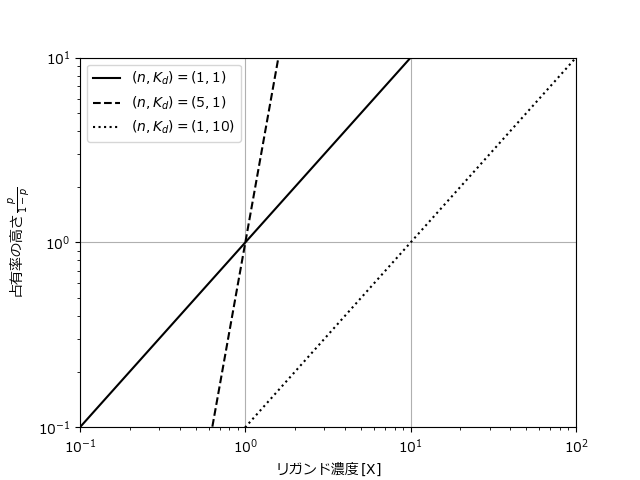
\includegraphics[width=10cm]{hill_plot.png}
  \caption{Hillの式に従う場合のHillプロット}
  \label{fig:hill_plot}
\end{figure}

具体的に受容体としてミオグロビン\footnote{筋肉に含まれる赤色のタンパク質.筋肉が運動して酸素を消費するときに備えて,普段は酸素を蓄える働きをする.}を,リガンドとして酸素を考える.
この場合にHillプロットを行うと,ミオグロビンのサイトの占有率は直線的になり(Hillの式に従い),$n=1$と求まる.
つまり,ミオグロビンは「最も単純なモデル」に従う受容体である.
一方で,受容体としてミオグロビンの代わりにヘモグロビン\footnote{赤血球に含まれる赤色のタンパク質.肺で受け取った酸素を全身に運搬する役割を担う.ミオグロビンは酸素の受け取り手の一つである.ちなみに,魚の赤身と白身の区別はヘモグロビンとミオグロビンの含有率に由来する.赤身の魚は長時間活発に泳ぐことができるが,これはヘモグロビンやミオグロビンが多いことで酸素を効率よく筋肉に回せるからである\cite{akami}.}を考えると,今度はHillプロットが直線的にならない部分が現れる.
それでもHillの式でフィッティングして$n$を求めると,$n=2$と$n=3$の間の非整数値となってしまう.
つまり,ヘモグロビンと酸素の結合はHillの式ではうまく説明できない.

\section{MWCモデル}

ヘモグロビンと酸素の結合を記述する有力なモデルとして,KNF(Koshland, N\'{e}methy, Filmer)モデルとMWC(Monod, Wyman, Changeux)モデルが知られている.
これらのモデルでは,Hillの式で無視されていた,受容体(ヘモグロビン)のサイトの一部にだけリガンド(酸素)が結合した状態も含めて取り扱う.
ここではとくにMWCモデルを紹介する.

\subsection{準備}

\begin{figure}[htbp]
  \centering
  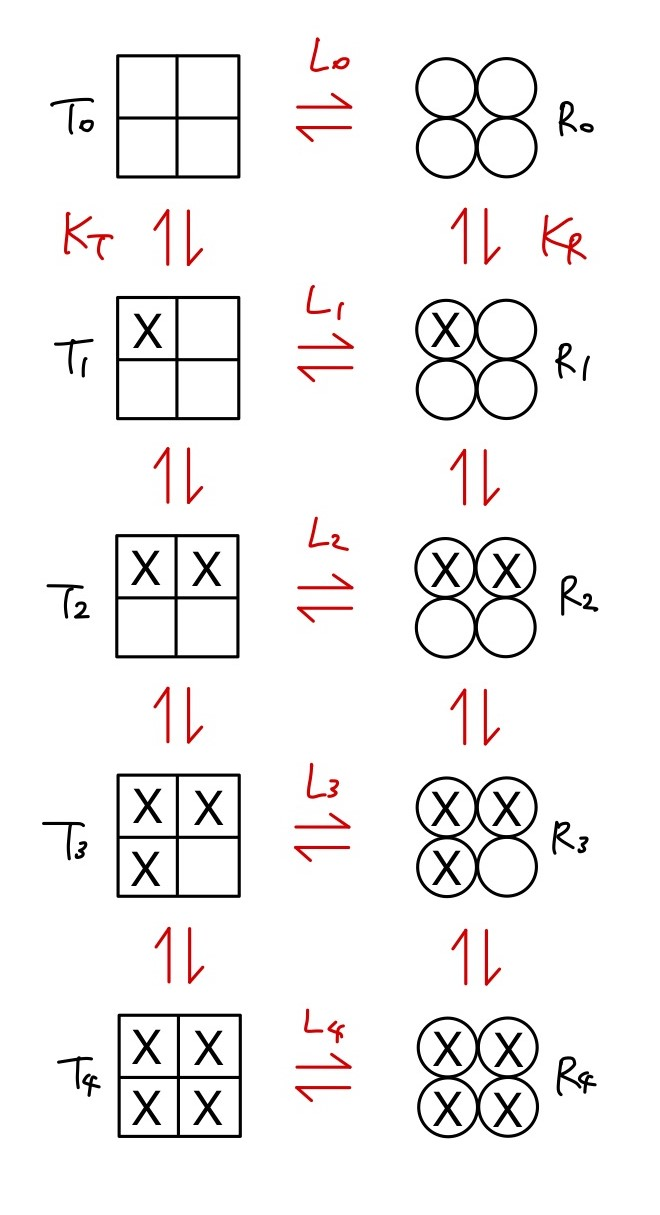
\includegraphics[width=5cm]{mwc_scheme.jpg}
  \caption{MWCモデルの概略図}
  \label{fig:mwc_scheme}
\end{figure}

MWCモデルでは,受容体が$n$個のサブユニットからなり,それぞれのサブユニットに一つずつリガンド結合サイトがあると考える.(ヘモグロビンと酸素の結合を考える際は$n=4$である.)
さらに,受容体が二つの状態(tense状態とrelaxed状態.それぞれT,Rと表す)の間を遷移すると考える\footnote{最近の研究ではヘモグロビンの状態としてT,Rの他にR2というものも見つかっており,実際のヘモグロビンの挙動はもっと複雑であると考えられている\cite{review}.}.
T状態の受容体に$i$個のリガンドが結合した状態を$\ce{T_{$i$}}$,R状態の受容体に$i$個のリガンドが結合した状態を$\ce{R_{$i$}}$と書く.
また,T(R)状態の受容体の空きサイトにリガンドが結合する反応の速度定数は$k_{\mathrm{on},\ce{T}}$($k_{\mathrm{on},\ce{R}}$),その逆反応は$k_{\mathrm{off},\ce{T}}$($k_{\mathrm{off},\ce{R}}$)で一定とする.
このとき,各反応の会合定数(解離定数の逆数)は
\begin{equation}
  K_{\ce{T}} = \frac{k_{\mathrm{on},\ce{T}}}{k_{\mathrm{off},\ce{T}}} \qquad K_{\ce{R}} = \frac{k_{\mathrm{on},\ce{R}}}{k_{\mathrm{off},\ce{R}}}
\end{equation}
となる(図\ref{fig:mwc_scheme}).

また,$n$個のサブユニットを区別し,どのような順番でもリガンドが結合できると仮定する.
たとえばリガンドが1つだけ結合した$\ce{T1}$は,実際には「どのサブユニットにリガンドが結合しているか」によって区別された$n$通りの状態を含むと考える.
これをもとに,$i=1,2,\cdots,n$に対して$\ce{T_$i-1$}$と$\ce{T_$i$}$の間の遷移を考える.
まず$\ce{T_$i-1$}$から$\ce{T_$i$}$への反応は,リガンドの結合していない$n-i+1$個のサイトで起こるので,速度定数は$(n-i+1)k_{\mathrm{on},\ce{T}}$となる.
一方でその逆反応は,リガンドの結合している$i$個のサイトで起こるので,速度定数は$ik_{\mathrm{off},\ce{T}}$となる.
$\ce{R_$i-1$}$と$\ce{R_$i$}$の間の遷移についても同様のことがいえる.

先ほどまではレート方程式を立てて定常状態を議論したが,ここでは簡単のため,すべての反応について化学平衡が成り立つと考えて平衡状態を議論する.
そのため,次が成り立つと考える:
\begin{align}
  (n-i+1)k_{\mathrm{on},\ce{T}}[\ce{T_$i-1$}][\ce{X}] &= ik_{\mathrm{off},\ce{T}}[\ce{T_$i$}] \\
  (n-i+1)k_{\mathrm{on},\ce{R}}[\ce{R_$i-1$}][\ce{X}] &= ik_{\mathrm{off},\ce{R}}[\ce{R_$i$}]
\end{align}
これより,
\begin{align}
  [\ce{T_$i$}] &= {}_n \mathrm{C}_i (K_{\ce{T}}[\ce{X}])^i [\ce{T0}] \label{Ti}\\
  [\ce{R_$i$}] &= {}_n \mathrm{C}_i (K_{\ce{R}}[\ce{X}])^i [\ce{R0}] \label{Ri}
\end{align}
がいえる.
加えて,すべての反応が平衡にあると考えるので,$\ce{T_$i$}$と$\ce{R_$i$}$の間の平衡も考える必要がある.
$\ce{T_$i$}$から$\ce{R_$i$}$への反応の速度定数を$l_{\ce{TR},i}$,その逆反応の速度定数を$l_{\ce{RT},i}$とおく.
このとき,この間の平衡定数を
\begin{equation}
  L_{i} = \frac{l_{\ce{RT},i}}{l_{\ce{TR},i}} = \frac{[\ce{T_$i$}]}{[\ce{R_$i$}]} \label{Li_def}
\end{equation}
とおく.

ただし,今まで考えてきた「すべての反応が平衡」という状況が実現するには条件がある.
それは,式\eqref{Li_def}に式\eqref{Ti}と式\eqref{Ri}を代入すると得られる式
\begin{equation}
  L_{i} = \frac{{}_n \mathrm{C}_i (K_{\ce{T}}[\ce{X}])^i [\ce{T0}]}{{}_n \mathrm{C}_i (K_{\ce{R}}[\ce{X}])^i [\ce{R0}]} = L_0 c^i \label{Li}
\end{equation}
である.ここで,
\begin{equation}
  c = \frac{K_{\ce{T}}}{K_{\ce{R}}}
\end{equation}
とおいた.
平衡定数$L_i$がこれを満たさないと3つの式\eqref{Ti},\eqref{Ri},\eqref{Li_def}が矛盾してしまうため,「すべての反応が平衡」という状態は存在しなくなる.
そのためここでは式\eqref{Li}も成り立つと考える.

\subsection{占有率の計算}
受容体のサイトの占有率は
\begin{equation}
  p = \frac{\sum_{i=0}^{n} i\qty([\ce{T_$i$}] + [\ce{R_$i$}])}{n\sum_{i=0}^{n} \qty([\ce{T_$i$}] + [\ce{R_$i$}])}
\end{equation}
である.
二項定理とその微分から得られる式
\begin{align}
  \sum_{i=0}^{n} {}_n \mathrm{C}_i x^i &= (1+x)^n \\
  \sum_{i=0}^{n} i\,{}_n \mathrm{C}_i x^i &= nx(1+x)^n-1
\end{align}
を用いると,
\begin{equation}
  \sum_{i=0}^{n} [\ce{T_$i$}] = \sum_{i=0}^{n} {}_n \mathrm{C}_i (K_{\ce{T}}[\ce{X}])^i [\ce{T0}] = \qty(1+K_{\ce{T}}[\ce{X}])^n [\ce{T0}] 
\end{equation}
\begin{equation}
  \sum_{i=0}^{n} [\ce{R_$i$}] = \sum_{i=0}^{n} {}_n \mathrm{C}_i (K_{\ce{R}}[\ce{X}])^i [\ce{R0}] = \qty(1+K_{\ce{R}}[\ce{X}])^n [\ce{R0}]
\end{equation}
\begin{equation}
  \sum_{i=0}^{n} i[\ce{T_$i$}] = \sum_{i=0}^{n} i\,{}_n \mathrm{C}_i (K_{\ce{T}}[\ce{X}])^i [\ce{T0}] = n K_{\ce{T}}[\ce{X}]\qty(1+K_{\ce{T}}[\ce{X}])^{n-1} [\ce{T0}] 
\end{equation}
\begin{equation}
  \sum_{i=0}^{n} i[\ce{R_$i$}] = \sum_{i=0}^{n} i\,{}_n \mathrm{C}_i (K_{\ce{R}}[\ce{X}])^i [\ce{R0}] = n K_{\ce{R}}[\ce{X}]\qty(1+K_{\ce{R}}[\ce{X}])^{n-1} [\ce{R0}] 
\end{equation}
がいえるので,
\begin{equation}
  x = K_{\ce{R}}[\ce{X}], \qquad cx = K_{\ce{T}}[\ce{X}]
\end{equation}
とおくと
\begin{equation}
  p = \frac{x(1+x)^{n-1} + L_0 cx (1+cx)^{n-1}}{(1+x)^n + L_0 (1+cx)^n} \label{mwc}
\end{equation}
が得られる.

しかし,この占有率がHillの式のような急峻なS字カーブを描くかというと,必ずしもそうではない.
たとえば,$L_0 \to 0$のとき
\begin{equation}
  p \to \frac{x}{1+x}
\end{equation}
となり,$L_0 \to \infty$のとき
\begin{equation}
  p \to \frac{cx}{1+cx}
\end{equation}
となるが,これらはいずれも「最も単純なモデル」で導いた形であり,S字にはならない.
そこで,Hill式のような曲線が現れる条件を考える.
まず,Hillの式の特徴として,リガンドの濃度が0のときに占有率の変化率が微小というものがある.
よって
\begin{equation}
  \left.\dv{p}{x}\right|_{x=0} = \frac{L_0 c + 1}{L_0 + 1} \ll 1
\end{equation}
が必要である.
これは
\begin{equation}
  L_0 \gg 1 , \qquad c \ll 1 \label{ggll}
\end{equation}
すなわち
\begin{equation}
  [\ce{T_0}] \gg [\ce{R_0}] ,\qquad K_{\ce{T}} \ll K_{\ce{R}}
\end{equation}
ということである.
つまり,リガンドが結合しないときは受容体はほとんどT状態にあるが,R状態の方がリガンドと結合しやすいという状況を意味する.
また式\eqref{Li}を考えると,式\eqref{ggll}が成り立つとは,$i$が大きくなるにつれて$L_i=L_0c^i$が小さくなるということでもある.
つまり,結合するリガンドの数が多いほどR状態の割合が増すという状況である.

このような状況が実現する(式\eqref{ggll}が成立する)という前提で,その後リガンドの濃度が上がったときに占有率が立ち上がる条件として,
\begin{equation}
  \left.\dv[2]{p}{x}\right|_{x=0} = \frac{nL_0 (1-c)^2 - (L_0 c^2 + 1)(L_0 + 1)}{(L_0 + 1)^2} > 0 
\end{equation}
が必要である.
これを変形すると
\begin{equation}
  n > \frac{(L_0 c^2 + 1)(L_0 + 1)}{L_0 (1-c)^2} \approx L_0 c^2 + 1 \label{ng}
\end{equation}
が得られる.
これらを満たすようなパラメータで数値計算すると,Hillの式のような曲線が得られる(図\ref{fig:mwc}(1)).


\begin{figure}[htbp]
  \centering
  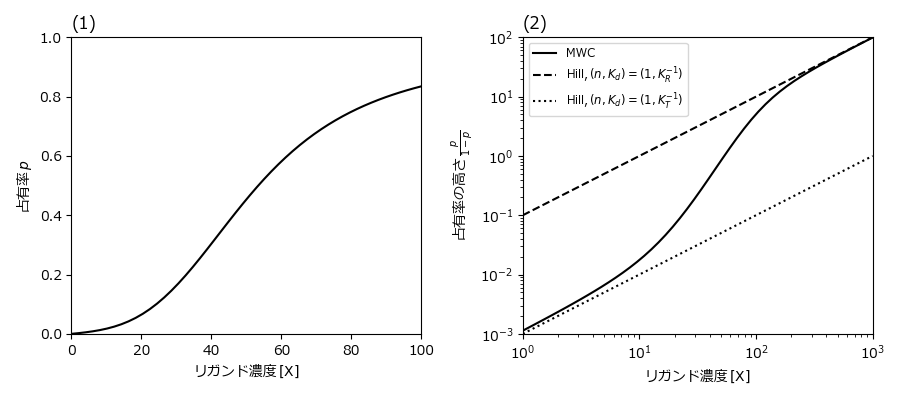
\includegraphics[width=14cm]{mwc.png}
  \caption{(1)MWCモデルによって得られる曲線($n = 4,\, K_{\ce{R}} = 0.1,\, L_0 = 1000,\, c = 0.01$)と(2)そのHillプロット(実線)および会合定数$K_{\ce{R}},K_{\ce{T}}$に対応する$n=1$のHillプロット(それぞれ破線,点線)}
  \label{fig:mwc}
\end{figure}

\subsection{Hillプロット}
MWCモデルで得られる曲線は,一般にHillプロットで直線にならず(図\ref{fig:mwc}(2)),ヘモグロビンと酸素の結合をうまく記述できることが知られている\footnote{ヘモグロビンは4量体なので$n=4$とすれば記述できる.}.
また図\ref{fig:mwc}(2)を見ると,MWCモデルのHillプロットはリガンド濃度が大きい極限と小さい極限で直線に漸近することが分かる.
ここではその理由と漸近線の意味を考える\footnote{この節では参考文献\cite{TBoC}の内容ではなく,私の考察を書いた.}.

まず,式\eqref{mwc}より
\begin{equation}
  \frac{p}{1-p} = x\frac{(1+x)^{n-1} + L_0 c(1+cx)^{n-1}}{(1+x)^{n-1} + L_0 (1+cx)^{n-1}} = x\frac{1+L_0c\qty(\frac{1+cx}{1+x})^{n-1}}{1+L_0\qty(\frac{1+cx}{1+x})^{n-1}}
\end{equation}
が分かる.
ここで$[\ce{X}] \ll 1$のとき$x \ll 1$であり,このとき
\begin{equation}
  \qty(\frac{1+cx}{1+x})^{n-1} \approx 1
\end{equation}
なので
\begin{equation}
  \frac{p}{1-p} \approx x\frac{1+L_0c}{1+L_0}
\end{equation}
がいえる.
さらに式\eqref{ggll}より,$1 \ll Lc  \ll L$であることを考えると,これはさらに
\begin{equation}
  \frac{p}{1-p} \approx cx = K_{\ce{T}}[\ce{X}] 
\end{equation}
と近似できる.
したがって
\begin{equation}
  \log{\frac{p}{1-p}} \approx  \log{[\ce{X}]} + \log{K_{\ce{T}}} \label{hill_t}
\end{equation}
となる.
つまり$[\ce{X}] \ll 1$でHillプロットは傾き1の直線になる.
さらに言えば,これはHillの式で$n=1,\,K_d=K_{\ce{T}}^{-1}$のときに対応する\footnote{$K_{\ce{T}}$は会合定数なので,その逆数$K_{\ce{T}}^{-1}$は解離定数を意味する.}.
よって,これはT状態の一段階反応に対応している.
物理的には,リガンドが少ない状況においてリガンドと受容体の反応はほぼ$\ce{T_0 + X <=> T_1}$が占めると解釈できる.

一方で$[\ce{X}] \gg 1$のとき$x \gg 1$であり,このとき
\begin{equation}
  \qty(\frac{1+cx}{1+x})^{n-1} \approx c
\end{equation}
なので
\begin{equation}
  \frac{p}{1-p} \approx x\frac{1+L_0c^n}{1+L_0c^{n-1}}
\end{equation}
がいえる.
さらに式\eqref{ggll}と式\eqref{ng}より,$n\ge 4$に対しては$1 \gg L_0c^{n-1}  \gg L_0c^{n}$である\footnote{式\eqref{ng}は$L_0c^2$が1と同程度かそれ未満のスケールであることを意味する.ここに$c$をかけると式\eqref{ggll}から$L_0 c^3 \ll 1$がいえるので,一般に$n\ge 4$に対して$1 \gg L_0 c^{n-1} \gg L_0 c^{n}$が成り立つ.もし$L_0c^2$が1未満のスケールなら$n=3$でも成り立ち,$L_0c$が1未満のスケールなら$n=2$でも成り立つ.}ことを考えると,$n \ge 4$のときこれはさらに
\begin{equation}
  \frac{p}{1-p} \approx x = K_{\ce{R}}[\ce{X}] 
\end{equation}
と近似できる.
したがって
\begin{equation}
  \log{\frac{p}{1-p}} \approx  \log{[\ce{X}]} + \log{K_{\ce{R}}} \label{hill_r}
\end{equation}
となる.
つまり$[\ce{X}] \gg 1$でもHillプロットは傾き1の直線になる.
さらに言えば,$n \ge 4$のときこれはHillの式で$n=1,\,K_d=K_{\ce{R}}^{-1}$のときに対応する.
よって,これはR状態の一段階反応に対応している.
物理的には,リガンドが多い状況においてリガンドと受容体の反応はほぼ$\ce{R_{$n-1$} + X <=> R_{$n$}}$が占めると解釈できる.

\subsection{応用}
MWCモデルが当てはまる例はヘモグロビンと酸素の結合以外にも確認されている.
有名な例としてバクテリアが挙げられる.
バクテリアは自分の栄養になる物質などの誘引物質を感知し,その濃度が高い方へ運動する.
これは走化性と呼ばれ,誘引物質が受容体に結合したことで発されるシグナルに応答することで実現している.
この誘引物質と受容体の結合も,MWCモデルがよく当てはまることが知られる.

\section{ヘモグロビンの役割}
これまでヘモグロビンと酸素の結合について数理的に考えてきた.
しかし,そもそもなぜヘモグロビンはミオグロビンとは違ってここまで複雑なことをやっているのだろうか.
その理由はヘモグロビンの働きにある.
ヘモグロビンは肺で酸素を効率よく受け取るために,肺ではできるだけ多くのサイトを酸素で埋めた方が良い.
一方で肺以外の部位では,酸素を効率よく手放して各組織に受け渡すために,占有率は極力低い方が良い.
アロステリック効果による占有率のS字カーブは,この両方を見事に実現している.

一方でミオグロビンは,ヘモグロビンから受け取った酸素を蓄える働きをするので,ヘモグロビンのサイトの占有率が低いときであっても高い占有率が求められる.
これは単純な反応による双曲線のカーブによって実現される.

また,ヘモグロビンに働くアロステリック効果は他にもある.
たとえばpHが低い状況では,ヘモグロビンが水素イオンと結合することで酸素との結合が起こりづらくなることが知られている(Bohr効果)\cite{bohr}.
この効果により,血中の二酸化炭素濃度が高いと,二酸化炭素が水と反応して水素イオンを放出する(pHを低くする)ため,ヘモグロビンは酸素を離しやすくなる.
一般に,肺では酸素濃度が高く二酸化炭素濃度が低いのに対し,組織では酸素濃度が低く二酸化炭素濃度が高い.
そのため,Bohr効果によってヘモグロビンは肺で酸素を結合して組織でそれを手放すという仕事をさらに効率的に行うことができる\footnote{この話は高校の生物(生物基礎)の教科書に載っている.}.

このように,生物は必要に応じてアロステリック効果を利用し,生命活動を適切に制御している.
その意味で,アロステリック効果はアロステリック制御とも呼ばれる.

\begin{thebibliography}{99}
  \bibitem{TBoC} 金子邦彦,澤井哲,高木拓明,古澤力.『細胞の理論生物学 ダイナミクスの視点から』.東京大学出版会,2020.
  
  \bibitem{PBoC} Phillips, R., Kondev, J., and Theriot, J. \textit{Physical Biology of the Cell}. Garland Science, 2008;邦訳:『細胞の物理生物学』.共立出版,2011.
  %笹井理生,伊藤一仁,千見寺浄慈,寺田智樹.

  \bibitem{akami} 魚食普及推進センター.「赤身魚と白身魚の違い そして・・・青魚と赤魚とは??」.\\
  \url{https://osakana.suisankai.or.jp/s-other/4923}, (参照 2022-4-7).

  \bibitem{review} Yuan, Y., Tam, M. F., Simplaceanu, V., and Ho, C. New Look at Hemoglobin Allostery. \textit{Chem. Rev.},  \textbf{115}(4): 1702-1724, 2015.

  \bibitem{bohr} Wikipedia. ``Bohr effect".\\
  \url{https://en.wikipedia.org/wiki/Bohr_effect}, (参照 2022-4-7).
\end{thebibliography}
\end{document}